Unse Programm implementiert ein MVC Pattern. Die Komponenten Model und Controller sind als Java Pakete schnell ersichtlich. Die View wird aber nicht in einem Java-Packet  ausprogramiert. Da wir JavaFx neutzen, wird die View durch JavaFx definiert. Die Implementierungsdetails findet man unter resources/mainWindow.fxml. Auch das Notification Packet könnte man zur View zählen.

Die wichtigsten Komponenten sieht man in der Abbildung Systemübersicht.
\begin{landscape}
\begin{figure}
  \centering
    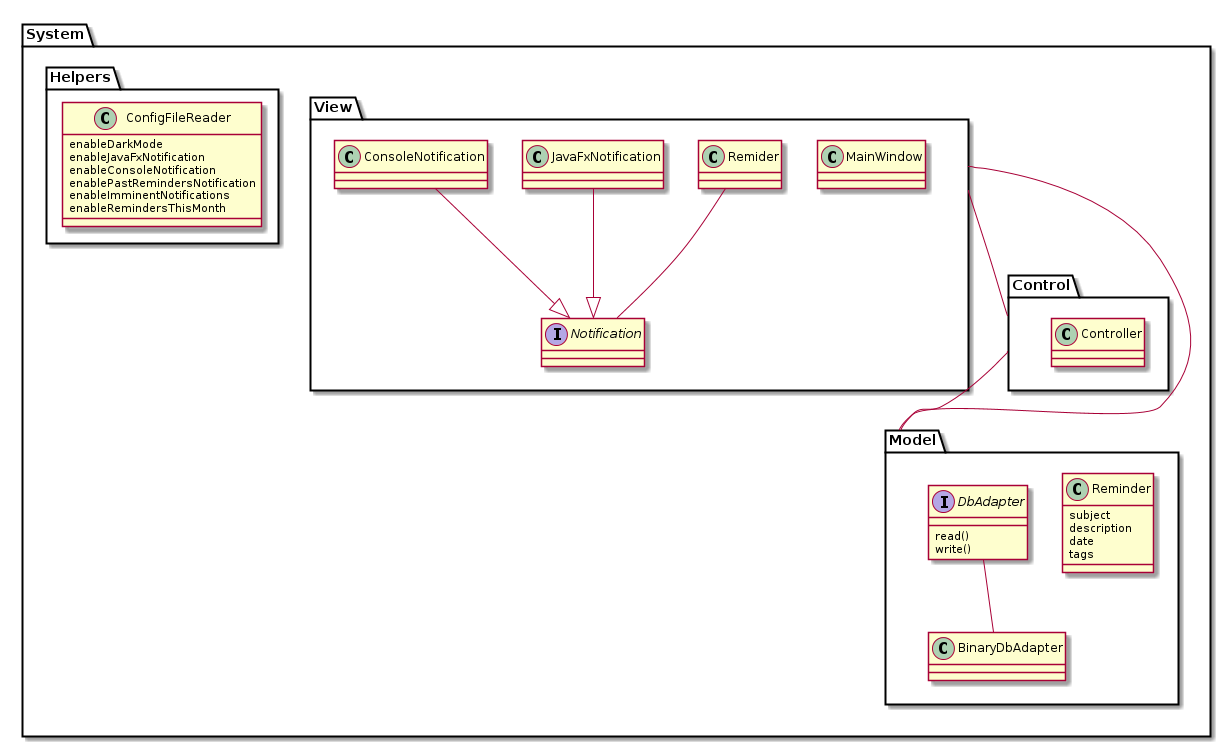
\includegraphics[width=1\textwidth]{../uml/uebersicht01.png}
  \caption{Systemübersicht}
  \label{fig:overview}
\end{figure}
\end{landscape}

Spezielle Aufmerksamkeit bedarf das Auslösen eines Reminders.
\subsection{Auslösen Notification}

Der Poller stösst regelmässig den NotificationHandler an.
In diesem werden Kriterien definiert, nach welchen die Reminders gefiltert werden.  Zum Beispiel alle Reminders, welche in der nächsten Stunde beginnen.



Dann wird über alle Reminders itteriert. Jedem Reminder, wird dabei der Filter an die NotifyIf() Funktion übergeben.
Der Reminder testet nun anhand des Filters selbstständig, ob des Kriterium zutrifft oder nicht. Dazu nutzt er seine meetsCriteria() Funktion.
Falls diese eine positive Antwort gibt, wird die doNotify Funktion aufgerufen. Diese lädt eine Liste mit den Notifications, welche im ConfigReader definiert wird. Jeder dieser Notifications wird der Reminder übergeben, welche die Notifications auslösen will. Dann wird die Notifications abgesendet.

\subsection{Konfiguration}
Die Konfigurationsmöglichkeiten sind im ConfigReader File zentral gelöst. Somit wird es später auch leicht möglich, über diese Klasse ein Konfigurationsfile  einzulesen, und die entsprechenden Komponenten zu konfigurieren.
